% The r-xla stack for the "anvl in one slide" slide.
% Same style as ../openxla-stack.tex: blue for what is ours, grey for the
% prebuilt plugins, dashed for the backend under evaluation.
\documentclass[tikz, border=8pt]{standalone}
\usetikzlibrary{arrows.meta, positioning, decorations.pathreplacing}

\begin{document}
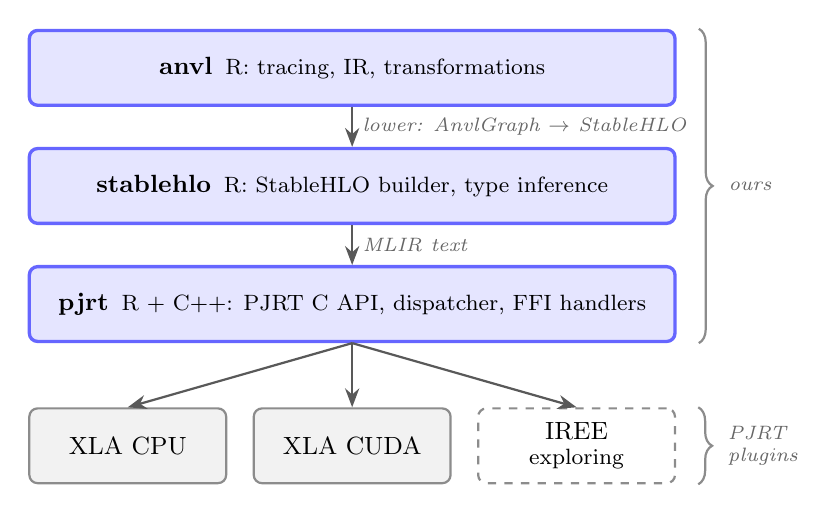
\begin{tikzpicture}[
  every node/.style={font=\small},
  box/.style={
    draw, rounded corners=3pt, thick,
    minimum height=0.95cm, align=center
  },
  ours/.style={box, fill=blue!10, draw=blue!60, very thick, minimum width=8.2cm},
  plugin/.style={box, fill=black!5, draw=black!45, minimum width=2.5cm},
  maybe/.style={box, draw=black!45, dashed, minimum width=2.5cm},
  arr/.style={-{Stealth[length=2.4mm, width=1.8mm]}, thick, draw=black!65},
  lab/.style={font=\scriptsize\itshape, text=black!60},
  brace/.style={decorate, decoration={brace, amplitude=5pt}, thick, draw=black!45}
]
  \node[ours] (anvl) at (0, 4.4)
    {\textbf{anvl}\enspace{\footnotesize R: tracing, IR, transformations}};
  \node[ours] (shlo) at (0, 2.9)
    {\textbf{stablehlo}\enspace{\footnotesize R: StableHLO builder, type inference}};
  \node[ours] (pjrt) at (0, 1.4)
    {\textbf{pjrt}\enspace{\footnotesize R + C++: PJRT C API, dispatcher, FFI handlers}};

  \node[plugin] (xcpu) at (-2.85, -0.4) {XLA CPU};
  \node[plugin] (xgpu) at (0, -0.4) {XLA CUDA};
  \node[maybe]  (iree) at (2.85, -0.4) {IREE\\[-2pt]{\footnotesize exploring}};

  \draw[arr] (anvl) -- node[right, lab] {lower: AnvlGraph $\to$ StableHLO} (shlo);
  \draw[arr] (shlo) -- node[right, lab] {MLIR text} (pjrt);
  \foreach \p in {xcpu, xgpu, iree} \draw[arr] (pjrt.south) -- (\p.north);

  \draw[brace] ([xshift=8pt]anvl.north east) -- ([xshift=8pt]pjrt.south east)
    node[midway, right=7pt, lab] {ours};
  \draw[brace] ([xshift=8pt]iree.north east) -- ([xshift=8pt]iree.south east)
    node[midway, right=7pt, lab, align=left] {PJRT\\plugins};
\end{tikzpicture}
\end{document}
